Given the goals outlined above, we propose the following experiment as an
initial evaluation of our proposed feasibility prediction approach. We use
model-based GUI test suites as our input suites and Java Swing applications as
Applications Under Test (AUTs). To support execution of these suites, we
develop a scalable and portable execution infrastructure. Below, we elaborate
on the experimental setup and planned analyses.

\subsection{ AUTs }

For this initial study, we chose two GUI-based Java Swing applications as
AUTs. While we acknowledge that choice of application platform and technology
may have some effects on experimental outcomes, in our case, Java tooling
for model-based test execution is far ahead of similar tooling for other
domains such as mobile and Web. We consider expansion of AUT domains an item
for future work.

Our first Java Swing application is the JabRef reference manager
\footnote{\url{http://jabref.sourceforge.net/}}, which features a complex
GUI built around extensive data entry and nearly 12 years of
open-source development. Our second application is
ArgoUML\footnote{\url{http://argouml.tigris.org/}}, a largely graphical
GUI-based Java application for constructing diagrams with connected
components. These applications represent real-world examples for model-based
testing. They also draw from multiple domains and use cases as GUI-based
applications.

\subsection{ Tools and Execution Infrastructure }

\begin{figure}[ht]
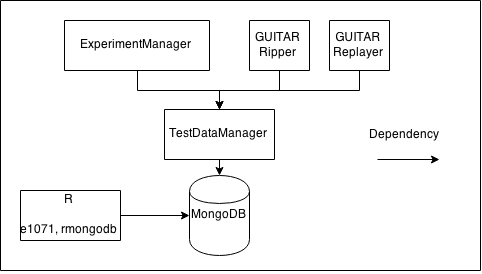
\includegraphics[width=\linewidth]{images/Tools.png}
\caption{Tool stack for experiments: Custom Java tools backed by a MongoDB database}
\label{fig:tools}
\end{figure}
\begin{figure*}[ht]
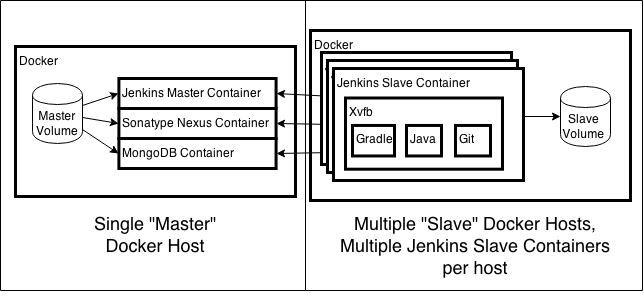
\includegraphics[width=\linewidth]{images/Infrastructure.png}
\caption{Infrastructure for experiment execution: Docker containers and volumes split over multiple hosts and coordinated by central components (Jenkins CI, Nexus repository, and MongoDB database)}
\label{fig:infrastructure}
\end{figure*}
\begin{figure}[ht]
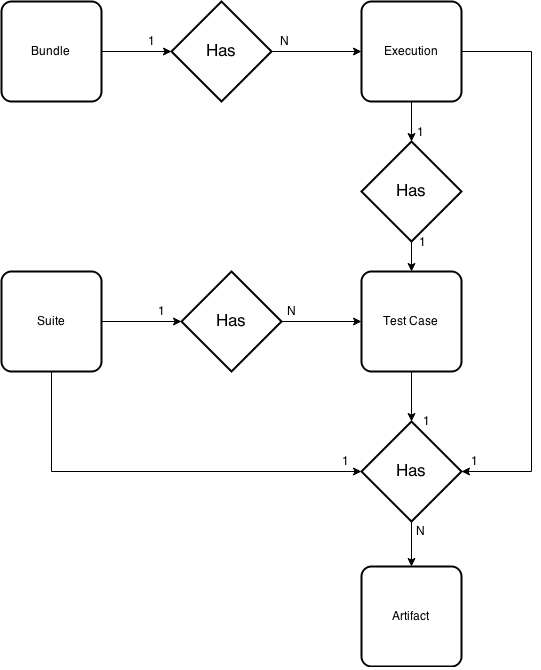
\includegraphics[width=\linewidth]{images/DataModel.png}
\caption{Data model for experiment results: Artifacts serialized into NoSQL DB and associated with test case, test suite, and test case executions; test cases grouped into suites, test executions grouped into bundles}
\label{fig:data}
\end{figure}


To carry our empirical evaluation of prediction techniques, we developed a reproducible,
reusable infrastructure from a combination of open-source and custom-built testing, continuous
integration (CI), and model-based testing tools. Figure \ref{fig:tools} shows our tool stack, and
Figure \ref{fig:Infrastructure} our runtime infrastructure for experiments.

First, we leveraged the Java toolchain of the GUITAR framework to generate and execute 
model-based test cases for each AUT. In particular, we use the GUITAR Ripper tool to
automatically extract a GUI Tree representation of the AUT. We then convert the GUI tree
to an Event-flow Graph (EFG), and the EFG into test suites. The GUITAR Replayer executes
test cases in each suite automatically. This approach for test case generation and replay is
elaborated in previous work \cite{XXX}.

In addition to the existing GUITAR Java toolchain, we developed two new, reusable tools for
this research. First, we developed TestDataManager, a tool for persistence of testing artifacts.
The TestDataManager, backed by the MongoDB NoSQL database, contains interfaces and utilities
for defining artifact conversion. The \texttt{TestDataManager} then stores artifacts in either a JSON-like
notation, or as raw binary files to MongoDB's GridFS filesystem. Figure \ref{fig:data} 
shows the underlying data model of the \texttt{TestDataManager}, which includes representations for both
test cases and test case executions. Test cases can be associated with one or more test suite and
one or more test execution. Bundles gather associated test case executions.

The testing process produces a continuous stream of artifacts at every step. In this experiment, we
rely on three input artifacts: test steps, GUI Tree, and EFG. Test cases are initially
defined by input files of test steps. The GUITAR Replayer depends on test steps defined in terms
of executable events, and events defined in terms of position in the GUI Tree. Consequently, the
Replayer draws from supporting information stored as GUI Tree and EFG artifacts shared by an
entire generated test suite. As output artifacts, we collect, store, and associate console
logs with each test case execution.

The \texttt{TestDataManager} and its associated data focus on maintaining artifacts and grouping them into
high-level abstractions common across testing techniques. We envision this tool supporting the storing
of test-related artifacts in general. To support the particular experiments of this work, we developed empirical
studies of software testing in the future. To focus on the particular
experiments of this work, we also developed the \texttt{ExperimentManager}. The \texttt{ExperimentManager}
supports higher-level analysis and comparison of artifacts with the following API:

\begin{itemize}
\item PostResults(TestDataManager, resultId, suiteId, Set bundleIds) - Given a set of execution bundles, categorize each test as feasible (always passing), infeasible (always failing), or inconsistent.
\item GetResultsObject(TestDataManager, resultId) - Return a results object previously constructed by a call to PostResults.
\item GenerateCombinationSuite(TestDataManager, suiteIdA, resultId, size) - Given a previously posted results object defined on a test suite A, randomly generate a new test suite {A\_combined} with a given size from combinations of feasible test cases in A.
\item addFeaturesForSuite(TestDataManager, suiteId) - For each test case in a given suite, extract and store a set of features from its the input artifacts.
\end{itemize}

Finally, we process apply machine learning algorithms and statistical analysis to artifacts in R. In particular, we use the \texttt{e1071} package
and its support for construction and analysis predictive binary classifiers. We import data from MongoDB with \texttt{rmongodb}.

\subsection{ Input and Combined Test Suites }

With the support of the ExperimentManager API and its underlying tools, we first generate model-based
test suites for each AUT (the "input" suite). Summary statistics for generated test suites are show in Table
\ref{tab:suites}. The GUI Tree and EFG artifacts produced by the GUITAR toolchain
can be used to generate a number of test suites based on event coverage criteria. For this experiment,
we chose to start with test
suites constructed to cover all sequences of length=1; therefore, each test suite is guaranteed to cover every event in
the EFG. We generate this suite by iterating over all events in the EFG, and constructing a test case for each
by finding a "path to root." (We define and elaborate on the sequence-length coverage test suite generation approach
in previous work \cite{YYY, ZZZ, AAA}.)
Each resulting test case starts with an event which is available upon application start,
and should proceed to the single event (i.e., the sequence of length 1) which the test case was designed to cover.
For JabRef, this "SL1" test suite includes 662 test cases (one for each of the 662 events in the EFG); and likewise,
500 test cases for ArgoUML.

To determine the feasibility of SL1 cases, we execute each test case 3 times and use the \texttt{ExperimentManager}'s
PostResults function to categorize each test case as feasible, infeasible, or inconsistent. For a test case to be feasible, it must
complete successfully all 3 out of the 3 executions. The test cases of the SL1 suite and their feasibility categorizations
from PostResults serve as training examples for a binary classifier of feasibility.

To evaluate the model's predictive ability, we derive from
the SL1 suite of each AUT an "SL1-C" suite of potential test cases which are combinations of feasible test cases of the
SL1 suite. 
We limit the scope of test case combinations to simple concatenation. To generate the SL1-C suite for each AUT, we randomly
select 1000 concatenations of two test cases (without replacement) from the corresponding SL1 suite. As these test cases
have not yet been executed, their feasibility is unknown at the time of prediction.

\subsection{ Feature Selection }

Test.

\subsection{ Binary Classifier }

Test.

\subsection{ Planned Analyses }

Given a model constructed from the input SL1 suite of each AUT, we consider how well this model can predict the
feasibility of unseen test cases from the SL1-C suite. We evaluate the effectiveness of the model based on its
false positive (FP) and false negative (FN) rates

